\documentclass[10.5pt,notitlepage]{article}
\usepackage[utf8]{inputenc}
\usepackage{amsthm}
\usepackage{amsmath}
\usepackage{amsfonts}
\usepackage{mathtools}
\usepackage{amsmath,amssymb}       
\usepackage{enumitem}   
\usepackage{enumerate}
\usepackage{verbatim} 
\usepackage{bbm}
\usepackage[backend=biber,style=apa]{biblatex}
\usepackage{csquotes}
\DeclareLanguageMapping{spanish}{spanish-apa}
\urlstyle{same}
\addbibresource{refer.bib}
\usepackage{etoolbox}
\patchcmd{\thebibliography}{\section*{\refname}}{}{}{}
\usepackage{hyperref}
\usepackage{booktabs}
\renewcommand{\qedsymbol}{$\blacksquare$}
\usepackage{makecell}
\usepackage[spanish]{babel}
\decimalpoint
\usepackage[letterpaper]{geometry}
\usepackage{mathrsfs}
\newenvironment{solucion}
  {\begin{proof}[Solución]}
  {\end{proof}}
\pagestyle{plain}
\usepackage{pdflscape}
\usepackage[table, dvipsnames]{xcolor}
\usepackage{longtable}
\usepackage{tikz}
\def\checkmark{\tikz\fill[scale=0.4](0,.35) -- (.25,0) -- (1,.7) -- (.25,.15) -- cycle;} 
\usepackage[bottom]{footmisc}
\usepackage{hyperref}
\usepackage{float}
\usepackage[utf8]{inputenc}
\usepackage{placeins}
\DeclareMathOperator{\Tr}{Tr}
\DeclareMathOperator{\diag}{diag}
\DeclareMathOperator{\argmax}{argmax}
\DeclareMathOperator{\argmin}{argmin}
\newcommand{\PP}{\mathbb{P}}
\newcommand{\Bb}{\mathcal{B}}
\newcommand{\RR}{\mathbb{R}}
\newcommand{\Ff}{\mathcal{F}}
\newcommand{\Ss}{\mathcal{S}}
\newcommand{\Aa}{\mathcal{A}}
\newcommand{\Jj}{\mathcal{J}}
\newcommand{\Cc}{\mathcal{C}}
\newcommand{\oo}{\varnothing}
\newcommand{\ee}{\varepsilon}
\newcommand{\Ee}{\mathcal{E}}
\newcommand{\EE}{\mathbb{E}}
\newcommand{\NN}{\mathbb{N}}
\newcommand{\Pp}{\mathcal{P}}
\newcommand{\Mm}{\mathcal{M}}
\newcommand{\lL}{\mathrm{L}}
\newcommand{\Cov}{\mathrm{Cov}}
\newcommand{\Var}{\mathrm{Var}}
\newcommand{\Ll}{\mathcal{L}}
\newcommand{\xx}{\mathbf{x}}
\newcommand{\abs}[1]{\left\lvert #1 \right\rvert}
\newcommand{\norm}[1]{\left\| #1 \right\|}
\newcommand{\inner}[1]{\left\langle #1 \right\rangle}
\newcommand{\corch}[1]{\left[ #1 \right]}
\newcommand{\kis}[1]{\left\{ #1 \right\}}
\newcommand{\pare}[1]{\left( #1 \right)}
\newcommand{\floor}[1]{\lfloor #1 \rfloor}

\theoremstyle{plain}

\newtheorem{thm}{Teorema}[section] % reset theorem numbering for each chapter
\newtheorem{defn}[thm]{Definición} % definition numbers are dependent on theorem numbers
\newtheorem{lem}[thm]{Lema} % same for example numbers
\newtheorem{remarkex}{Observación}
\newenvironment{rem}
  {\pushQED{\qed}\renewcommand{\qedsymbol}{$\triangle$}\remarkex}
  {\popQED\endremarkex}

\usepackage{geometry}
\usepackage{mathtools}
\usepackage{enumitem}
\usepackage{framed}
\usepackage{amsthm}
\usepackage{thmtools}
\usepackage{etoolbox}
\usepackage{fancybox}

\newenvironment{myleftbar}{%
\def\FrameCommand{\hspace{0.6em}\vrule width 2pt\hspace{0.6em}}%
\MakeFramed{\advance\hsize-\width \FrameRestore}}%
{\endMakeFramed}
\declaretheoremstyle[
spaceabove=6pt,
spacebelow=6pt
headfont=\normalfont\bfseries,
headpunct={} ,
headformat={\cornersize*{2pt}\ovalbox{\NAME~\NUMBER\ifstrequal{\NOTE}{}{\relax}{\NOTE}:}},
bodyfont=\normalfont,
]{exobreak}

\declaretheorem[style=exobreak, name=Ejercicio,%
postheadhook=\leavevmode\myleftbar, %
prefoothook = \endmyleftbar]{exo}
\usepackage{graphicx}
\graphicspath{ {images/} }
\title{Tarea 5: Introducción a Ciencia de Datos.}

\author{Rojas Gutiérrez Rodolfo Emmanuel}

\begin{document}
\maketitle


\section{Introduction}
A lo largo de esta tarea, \(M_{n\times m}(\RR)\) denota el espacio de todas las matrices de dimensión \(n\times m\) con coeficientes en los reales, adicionalmente si \(A \in M_{n\times m}(\RR)\) entonces \(A'\) denota a la matriz transpuesta de \(A\).

\setcounter{exo}{0}

\begin{exo}

\end{exo}
\begin{solucion}
Para este ejercicio, se empleo el conjunto de datos siguiente:\footnote{Los datos al completo, pueden ser consultados en \(R\).}
\begin{table}[H]
        \centering
        \begin{tabular}{@{}l@{\hskip 0.3in}r@{\hskip 0.3in}r@{\hskip 0.3in}r@{\hskip 0.3in}r@{}}
        \toprule
        \(MC\)&  \(VC\)&  \(LO\)&  \(NO\)&  \(SO\)\\ 
        \midrule          
        77&  82&  67&  67&  81\\
        63&  78&  80&  70&  81\\
        75&  73&  71&  66&  81\\
        55&  72&  63&  70&  68\\
        63&  63&  65&  70&  63\\
        53&  61&  72&  64&  73\\
        \(\vdots\)& \(\vdots\)& \(\vdots\)& \(\vdots\)& \(\vdots\)\\
        5&  30&  44&  36&  18\\
        12&  30&  32&  35&  21\\
        5&  26&  15&  20&  20\\
        0&  40&  21&  9&  14\\
        \end{tabular}
        \caption{Datos de puntuaciones de 88 estudiantes en \(5\) exámenes de 5 materias, 2 de ellos hechos a libro abierto y los restantes a libro cerrado.}
        \label{tab:1}
\end{table}
Es importante comentar que para \(i \in \kis{1, \hdots, 88}\), el renglón \(i\) de la tabla de datos \ref{tab:1} corresponde a las calificaciones del estudiante \(i\), en cada uno de los \(5\) exámenes presentados, adicionalmente, se tiene que las columnas \(MC\) y \(VC\) son las columnas que corresponden a los exámenes que fueron realizados a libro abierto. Ahora, sea \(X \in M_{88 \times 5}(\RR)\) aquella matriz de datos cuyas filas y columnas coinciden con las filas y columnas de la tabla de datos \ref{tab:1} y, suponga que cada observación de \(5\) estudiantes proviene de una misma distribución \(5\)-variada, con matriz de covarianzas \(\Sigma\) la cual se desconoce. Con este contexto, se pretende encontrar con fines de evaluación aquella combinación de pesos \(\kis{\omega_1, \hdots, \omega_5}\) que máximize la variabilidad en el conjunto de calificaciones, al proyectar las mismas mediante un promedio ponderado de la forma\footnote{En el artículo se menciona que se consideran solamente pesos escalados, tales que la suma de los cuadrados de los mismos, sea igual a uno.}
\begin{equation}\label{weighted}
 \omega_1 X_{i1} +\hdots+\omega_{5}X_{i5}, \text{ con } i \in \kis{1, \hdots, 88},
\end{equation}
lo cual, permitiría resumir de la mejor forma posible el desempeño de cada estudiante a través de los 5 exámenes y, diferenciarlo del rendimiento de los demás estudiantes. Como puede imaginar, existen infinidad de opciones para elegir los pesos anteriores, no obstante, muchas de ellas no permitan hacer diferencia alguna entre los estudiantes, por ejemplo, uno podría dar todo el peso al examen \(SO\), es decir, uno podría elegir los pesos \((\omega_1, \hdots, \omega_5)\) como \((0,0,0,0,1)\), no obstante, si a todos los alumnos les fuera muy bien o muy mal en dicho examen no se estaría haciendo distinción alguna entre ellos. Sin embargo, no debemos rompernos la cabeza desarrollando un algoritmo nuevo para determinar los pesos \((\omega_1, \hdots, \omega_5)\) necesarios para llevar a cabo nuestro cometido, pues, por lo visto en el tema de componentes principales, se sabe que el conjunto de pesos \((\omega_1, \hdots, \omega_5)\) que maximiza la variabilidad en el conjunto de datos proyectados mediante el promedio ponderado \ref{weighted}, puede elegirse como un vector propio \((\omega_1, \hdots, \omega_5)\) de \(\Sigma\) con norma \(1\) y asociado a su mayor valor propio, sin embargo, dado que se desconoce el valor de \(\Sigma\), se debe emplear en su lugar a la matriz de covarianzas muestral
\begin{equation}\label{teodioroger}
  S = \frac{X_{c}'X_{c}}{88},  
\end{equation}
donde, \(X_{c}\) representa a la matriz de datos \(X\) centrada. Este detalle hace una diferencia importante, pues, al ser \(S\) una estimación de \(\Sigma\) entonces \(S\) depende de los valores de la muestra \(X\), es decir, si hubiésemos observado a otros \(88\) alumnos presentar los exámenes y, sus calificaciones se distribuyeran de la misma manera que la de los \(88\) alumnos observados, muy posiblemente obtendríamos una muestra distinta a la presentada en la tabla de datos \ref{tab:1} y, por ende, también se debería obtener un valor de \(S\) distinto, de este modo, al calcular los pesos \((\omega_1, \hdots, \omega_5)\) como un vector propio de \(S\) con norma \(1\) asociado al mayor valor propio de \(S\), se obtiene un vector de pesos \(\hat{\omega}_1, \hdots, \hat{\omega}_5\) el cual depende del valor de la muestra y, por lo tanto, para cada \(i \in \kis{1,\hdots,5}\) la cantidad \(\hat{\omega}_i\) tiene asociada a ella cierta variabilidad. Ahora, una pregunta natural es: ¿Cómo podemos estimar esta variabilidad en cada una de las componentes del vector \(\hat{\omega}_1, \hdots, \hat{\omega}_5\)? La respuesta, mediante remuestreo Bootstrap aplicando el siguiente algoritmo:
\begin{itemize}\label{it.1}
    \item[\textit{1.}] Para \(n \in \kis{1, \hdots, 10000}\) se elige una muestra con reemplazo de las \(88\) filas de \(X\) de tamaño \(88\), con lo que, se forma una matriz \(X^{(n)} \in M_{88 \times 5}(\RR)\) cuyas filas son precisamente las filas obtenidas en el muestreo previo. 
    \item[\textit{2.}] Se calcula la matriz de covarianzas muestral para los datos en la matriz \(X^{(n)}\), como:
    \[S^{(n)} = \frac{X_{c}^{(n)}'X_{c}^{(n)}}{88},\]
    donde, \(X_{c}^{(n)}\) representa a la matriz \(X^{(n)}\) con sus datos centrados. Posteriormente, se obtiene \((\hat{\omega}_{1}^{(n)},\hdots, \hat{\omega}_{5}^{(n)})\), como un vector propio de \(X^{(n)}\) con norma \(1\) asociado al mayor valor propio de \(S^{(n)}\).
     \item[\textit{3.}] Se almacenan los valores \((\hat{\omega}_{1}^{(n)},\hdots, \hat{\omega}_{5}^{(n)})\) como la \(n\)-ésima columna de una matriz \(FC \in M_{5\times 10000}(\RR)\). Finalmente, si \(n = 10000\) el algoritmo acaba y obtenemos una matriz \(FC \in M_{5\times 10000}(\RR)\), cuya \(i\)-ésima fila consiste en \(10000\) estimaciones bootstrap del peso \(\omega_i\), con \(i\in \kis{1, \hdots,5}\). En otro caso, regrese al paso \textit{1}. 
\end{itemize}
Ahora, el algoritmo anterior posee un problema, dado que los vectores propios calculados en cada iteración no son únicos, pues, al multiplicar un vector propio de norma \(1\) por menos uno, se obtiene un vector propio con norma \(1\) y asociado al mismo valor propio, entonces, se adoptó el criterio de considerar únicamente aquellos muestreos en los cuales la primer coordenada de pesos estimados sea positiva, esto con el fin de poder reproducir los resultados en \textcite{diaconis_computer-intensive_1983}.\footnote{Además, de haber sido una recomendación del Dr. Quiroga.} Así, la matriz \(FC\) que resultó tras utilizar el algoritmo en \ref{it.1}, en realidad tiene dimensión \(5 \times 9534\). Por ende, dado \(i \in \kis{1, \hdots, 5}\) se tiene que la fila \(i\)-ésima de \(FC\), la cual se denotara por \(FC_i\), consiste en \(9534\) estimaciones Bootstrap para el peso \(\omega_i\) necesario para maximizar la variabilidad en los datos proyectados \eqref{weighted}, por lo que, una forma de obtener un estimador de la variabilidad de la estimación de este peso, es la desviación estándar muestral de \(FC_i\) y una estimación puntual de este peso estaría dada por el promedio de los datos en \(FC_i\), bajo esta idea se construyo Tabla presentada en el Cuadro \ref{tab:2}:
\begin{table}        
        \centering
        \begin{tabular}{@{}l@{\hskip 0.3in}r@{\hskip 0.3in}r@{\hskip 0.3in}r@{}}
            \toprule
             & Estimación Puntual & Estimación de la desv. estándar& \substack{\text{Valor estimado usando la matriz}\\ \text{de covarianzas \(S\) de \(X\)}.} \\
            \midrule
            \(\omega_1\) & 0.500 &  0.0560&   0.5054\\
            \(\omega_2\) & 0.3665 &   0.0416& 0.3683\\ 
            \(\omega_3\) & 0.3439 &  0.0290&  0.3457\\
            \(\omega_4\) & 0.4518 &  0.0393&  0.4511\\ 
            \(\omega_5\) & 0.5328 &  0.0454&  0.5347\\
            \bottomrule
        \end{tabular}
        \caption{Estimaciones puntuales y de variabilidad de los pesos \((\omega_1, \hdots, \omega_5)\), que generan la mayor variabilidad posible en el conjunto de datos proyectados.}
        \label{tab:2}
\end{table}
Cabe destacar que, la última columna en la Tabla presentada en el cuadro \ref{tab:2}, corresponde a la estimación que se habría obtenido al calcular los pesos deseados, como un valor propio de \(S\) con norma \(1\) asociado al valor propio más grande de \(S\),\footnote{Con \(S\) como en \eqref{teodioroger}.} de este modo, al comparar las columnas uno y tres de la tabla \ref{tab:2} puede ver que dichas estimaciones, y las estimaciones Bootstrap son muy similares. Por último, haciendo uso de los datos de la Tabla \eqref{tab:2}, se replico una de las gráficas presentadas en \textcite{diaconis_computer-intensive_1983}, la cual se presenta en la Figura \ref{fig:1}. En esta gráfica se puede observar lo que ya se vislumbraba en la segunda columna de la Tabla \ref{tab:2}, es decir, que la variabilidad de las estimaciones bootstrap para el vector de pesos es baja.
\begin{figure}[htb]
    \centering
    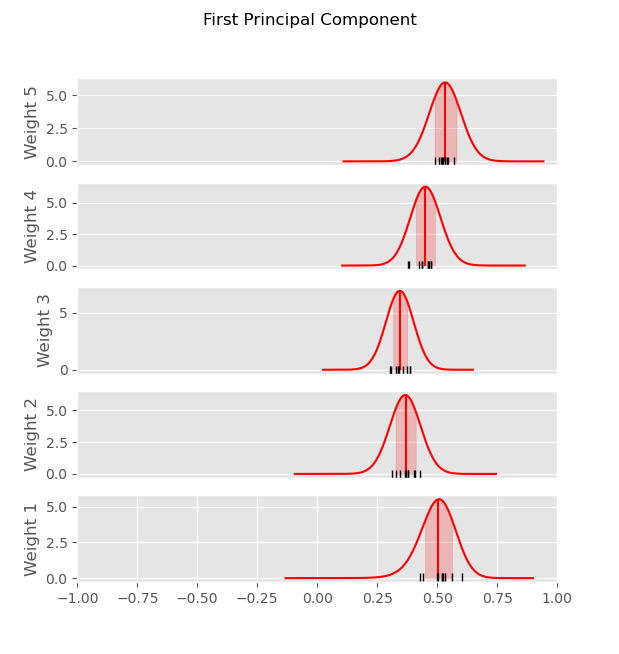
\includegraphics[scale = 0.5]{Figure_9.png}
    \caption{En linea roja solida se presentan las densidades por kernel de las 5 filas de \(FC\), en otras palabras, las densidades por kernel de las estimaciones bootstrap de cada uno de los 5 pesos, igualmente, en lineas rojas solidas verticales puede ver los valores correspondientes de la tercer columna, de la Tabla \ref{tab:2}, para cada uno de los pesos \((\omega_1, \hdots, \omega_5)\), por otro lado, el área sombreada en color rojo representa la porción del área bajo la curva que se encuentra a más menos una desviación estándar, segunda columna de la Tabla \ref{tab:2}, del valor marcado en linea roja, finalmente, en marcas negras se presentan algunas de las estimaciones bootstrap hechas para cada uno de los pesos.}
    \label{fig:1}
\end{figure}
Finalmente, en \textcite{diaconis_computer-intensive_1983}, se menciona que la segunda componente principal de \(\Sigma\) es el vector de pesos \((w_1, \hdots, w_5)\) que, sujeto a la restricción de independencia, genera la segunda mayor diferencia entre los alumnos, al proyectar con estos pesos los datos de calificaciones como en \eqref{weighted}. Sin embargo, para encontrar estos pesos nuevamente nos encontramos ante el problema de que la matriz \(\Sigma\) es desconocida y, por ende, no podemos calcular esta segunda componente simplemente obteniendo un vector propio normalizado de \(\Sigma\), correspondiente a su segundo valor propio más grande, no obstante, para estos pesos es posible realizar  un análisis análogo al realizado para la primer componente de la siguiente forma. Primero, una primer estimación para estos pesos puede obtenerse al calcular el vector propio de \(S\) con norma \(1\) asociado al segundo valor propio más grande de \(S\), ahora, sabemos que esta estimación trae consigo incertidumbre, la cual podemos cuantificar de cierto modo al modificar el algoritmo bootstrap dado para la primer componente principal de la siguiente manera:\footnote{Con el fin de que los remuestreos de filas, con los que se obtienen las estimaciones bootstrap para la primer y segunda componente principales en cada iteración, sean iguales se debe correr ambos algoritmos al mismo tiempo.} 
\begin{itemize}
    \item[\textit{1.}] Para \(n \in \kis{1, \hdots, 10000}\) se elige una muestra con reemplazo de las \(88\) filas de \(X\) de tamaño \(88\), con lo que, se forma una matriz \(X^{(n)} \in M_{88 \times 5}(\RR)\) cuyas filas son precisamente las filas obtenidas en el muestreo anterior. 
    \item[\textit{2.}] Se calcula la matriz de covarianzas muestral para los datos en la matriz \(X^{(n)}\), como:
    \[S^{(n)} = \frac{X_{c}^{(n)}'X_{c}^{(n)}}{88},\]
    donde, \(X_{c}^{(n)}\) representa a la matriz \(X^{(n)}\) con sus datos centrados. Posteriormente, se obtiene \((\hat{w}_{1}^{(n)},\hdots, \hat{w}_{5}^{(n)})\), como un vector propio de \(X^{(n)}\) con norma \(1\) asociado al segundo mayor valor propio de \(S^{(n)}\).
     \item[\textit{3.}] Se almacenan los valores \((\hat{w}_{1}^{(n)},\hdots, \hat{w}_{5}^{(n)})\) como la \(n\)-ésima columna de una matriz \(SC \in M_{5\times 10000}(\RR)\). Finalmente, si \(n = 10000\) el algoritmo acaba y obtenemos una matriz \(SC \in M_{5\times 10000}(\RR)\), cuya fila \(i\)-ésima consiste en \(10000\) estimaciones bootstrap del peso \(w_i\), con \(i \in \kis{1, \hdots,5}\). En otro caso, regrese al paso \textit{1}. 
\end{itemize}
Ahora, el algoritmo previo posee el mismo problema que el primer algoritmo dado en \ref{it.1}, por lo que, también se adopto el criterio de considerar únicamente aquellos muestreos en los cuales la primer coordenada de pesos estimados sea positiva, esto con el fin de poder reproducir los resultados en \textcite{diaconis_computer-intensive_1983}. De este modo, la matriz \(SC\) que resultó tras utilizar el algoritmo tiene dimensión \(5 \times 7649\). Por ende, dado \(i \in \kis{1, \hdots, 5}\) se tiene que la fila \(i\)-ésima de \(SC\), la cual se denotara por \(SC_i\), consiste en \(7649\) estimaciones Bootstrap para el peso \(w_i\) que genera la segunda mayor diferencia variabilidad en los datos proyectados \eqref{weighted}, sujeto a la restricción de independencia, por lo que, una forma de obtener un estimador de la variabilidad de la estimación de este peso, es la desviación estándar muestral de \(SC_i\) y una segunda estimación puntual de este peso estaría dada por el promedio de los datos en \(SC_i\), con esto en mente, se construyo Tabla presentada en el Cuadro \ref{tab:3}:
\begin{table}[H]        
        \centering
        \begin{tabular}{@{}l@{\hskip 0.3in}r@{\hskip 0.3in}r@{\hskip 0.3in}r@{}}
            \toprule
             Pesos& Estimación Puntual & Estimación de la desv. estándar& \substack{\text{Valor estimado usando la matriz}\\ \text{de covarianzas \(S\) de \(X\)}.} \\
            \midrule
            \(w_1\) & 0.7434 &  0.0767&   0.7487\\
            \(w_2\) & 0.1918 &   0.1256& 0.2074\\ 
            \(w_3\) & -0.0786 &  0.0631&   -0.0759\\
            \(w_4\) & -0.3080&  0.1115&   -0.3009\\ 
            \(w_5\) &  -0.5082 &  0.1151&   -0.5478\\
            \bottomrule
        \end{tabular}
        \caption{Estimaciones puntuales y de variabilidad de los pesos \((w_1, \hdots, w_5)\), que generan la segunda mayor variabilidad posible en el conjunto de datos proyectados, sujeto a la restricción de independencia.}
        \label{tab:3}
\end{table}
Es importante resaltar que la última columna en la Tabla presentada en el cuadro \ref{tab:3}, corresponde a la estimación que se habría obtenido al calcular los pesos deseados, como el valor propio de \(S\) con norma \(1\) asociado al segundo valor propio más grande de \(S\), por lo que, se concluye que las dos estimaciones puntuales dadas son similares en los \(5\) casos.\footnote{Con \(S\) como en \eqref{teodioroger}.} Finalmente, se recreo con los datos de la Tabla \ref{tab:3} la segunda gráfica presentada en \textcite{diaconis_computer-intensive_1983}, la cual se expone en la Figura \ref{fig:2}. De este modo, al comparar las gráficas en \ref{fig:1} y \ref{fig:2} se advierte que, existe mayor variabilidad en los pesos estimados mediante la segunda componente principal, lo cual puede corroborarse al ver las segundas columnas de las Tablas \ref{tab:2} y \ref{tab:3}, por último, en el artículo se comenta que el promedio obtenido con los pesos estimados con el segundo componente principal, puede interpretarse como la diferencia entre un promedio de pruebas a libro abierto y un promedio de pruebas a libro cerrado, ahora, los pesos asociados a las pruebas a libro cerrado son \(\kis{w_3, w_4, w_5}\), mientras que, los pesos asociados a las pruebas a libro cerrado son \(\kis{w_1, w_2}\),\footnote{Ver relación en \eqref{weighted} sustituyendo \(\omega's\) por \(w's\).} observe que, esta idea se ver reforzada con los resultados en las gráfica presentadas en la Figura \ref{fig:2}, pues, las distribuciones bootstrap de los pesos en \(\kis{w_4, w_5}\) y en \(\kis{w_1, w_2}\) parecen estar perfectamente separadas, caracterizando a los exámenes a libro cerrado y abierto.
\begin{figure}[htb]
    \centering
    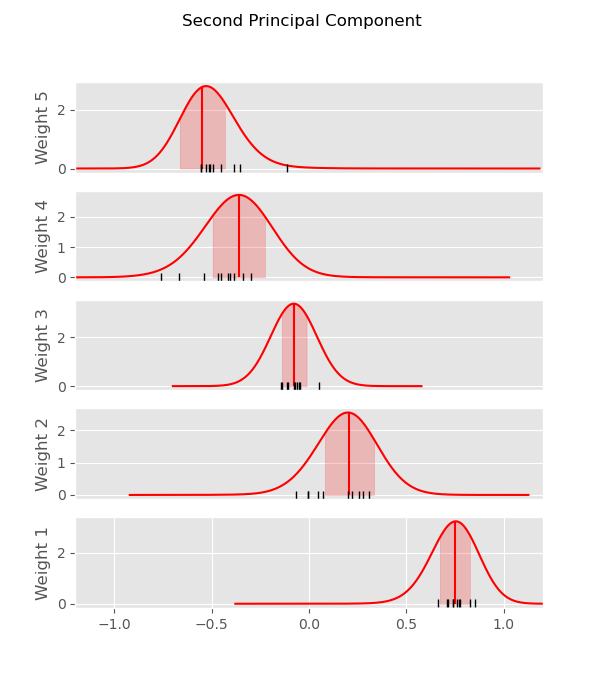
\includegraphics[scale = 0.5]{Figure_16.png}
    \caption{En linea roja solida se presentan las densidades por kernel de las 5 filas de \(SC\), en otras palabras, las densidades por kernel de las estimaciones bootstrap de cada uno de los 5 pesos, igualmente, en lineas rojas solidas verticales puede ver los valores correspondientes de la tercer columna en la Tabla \ref{tab:3} a cada uno de los pesos \((w_1, \hdots, w_5)\), por otro lado, el área sombreada en color rojo representa la porción del área bajo la curva que se encuentra a más menos una desviación estandár, segunda columna de la Tabla \ref{tab:3}, del valor marcado en linea roja, finalmente, en marcas negras se presentan algunas de las estimaciones bootstrap hechas para cada uno de los pesos.}
    \label{fig:2}
\end{figure}
Como comentario final, se destaca que la aplicación del remuestreo bootstrap en este problema, es una manera ingeniosa de cuantificar la incertidumbre en las estimaciones dadas, por lo que, se cree que es importante conocer diversas herramientas estadísticas, pues, la combinación de ellas puede resultar en análisis mucho más completos, como en este caso, en el que se ha combinado un análisis de componenetes principales, con una aplicación del remuestreo Bootstrap. 

\begin{rem}
En el script adjunto, puede encontrar intervalos de confianza al \(95\%\) para cada uno de los pesos calculados en el ejercicio, todos ellos construidos con los cuantiles muéstrales de las estimaciones bootstrap. Se comenta esto, pues, por cuestiones de espacio y tiempo no se alcanzo a incluir los mismos en este documento.
\end{rem}
\end{solucion}

  




%%%%%%%%%%%%%%%%%%%%%%%%%%%%%%%%%%%%%%%%%%%%%%%%%%%%%%%%%%%%%%%%%%%%%%%%%%%%%%%%%%%%%
\begin{exo}

\end{exo}
\textbf{a)}
\begin{solucion}
Dados \(n\) y \(k\) dos números naturales tales que \(1 \leq k \leq n\), defina \(S(n,k)\) como el número de formas de acomodar \(n\) objetos en \(k\) grupos disjuntos y no vacíos, con la convención de que \(S(n-1,n) = 0\), lo cual tiene sentido pues, el número de formas de acomodar \(n-1\) objetos en \(n\) grupos disjuntos y no vacíos, debe ser cero, dado que no existen suficientes objetos como para formar el número de grupos deseado, adicionalmente, otra convención que será adoptada es que \(S(0,0) = 1\). Con este contexto en mente, se argumentará el porque igualdad: 
\[
S(n,k) = S(n-1,k-1) + k S(n-1,k),
\]
es valida para cualesquiera dos números naturales \(n\) y \(k\) que cumplan la desigualdad \(1 \leq k \leq n\). Para ello, sean \(n\) y \(k\) dos números naturales tales que \(1 \leq k \leq n\) y, suponga que tiene \(n\) objetos los cuales etiqueta de la siguiente forma \(\kis{o_1, \hdots, o_n}\), entonces, note que existen únicamente dos maneras de formar \(k\) grupos no vacíos y disjuntos a partir de estos \(n\) objetos:
\begin{enumerate}
    \item[\textit{1}.] Seleccionar el primer grupo como \(\kis{o_n}\), con lo que, resta por acomodar en \(k - 1\) grupos disjuntos y no vacíos los sobrantes \(n-1\) objetos en \(\kis{o_1, \hdots, o_{n-1}}\), lo cual, por definición de \(S(n-1,k-1)\) puede hacerse de exactamente \(S(n-1, k-1)\) formas distintas. Así:
    \begin{align*}
        &\text{Existen \(S(n-1, k-1)\) formas distintas de acomodar los \(n\) objetos en \(k\) grupos,}\\
        &\text{cuando uno de los grupos es \(\kis{o_n}\).}
    \end{align*}
    \item[\textit{2}.] Que ninguno de los \(k\) grupos sea \(\kis{o_n}\), con lo que, \(\kis{o_{n}}\) debe ser un subconjunto propio de alguno de los \(k\) grupos en los que se particione el conjunto \(\kis{o_1, \hdots, o_n}\),\footnote{Pues, en otro caso el elemento \(o_n\) no se encontraría en ninguno de los \(k\) grupos en los que se particiono el conjunto \(\kis{o_1, \hdots, o_n}\), lo cual sería contradictorio.} así, si removemos el objeto \(o_n\) del grupo al que pertenece, dicho grupo sigue siendo no vacío pues \(\kis{o_n}\) es un subconjunto propio de tal grupo y, por ende, se obtiene una separación en \(k\) grupos  disjuntos no vacíos del conjunto \(\kis{o_1, \hdots, o_{n-1}}\), además, note que si se tiene una partición en \(k\) grupos disjuntos no vacíos del conjunto \(\kis{o_1, \hdots, o_{n-1}}\), entonces, al agregar a cualquiera de estos grupos el elemento \(o_{n}\), se obtiene una partición del conjunto \(\kis{o_1, \hdots, o_n}\) en \(k\) grupos disjuntos no vacíos. De este modo, el problema de encontrar todas las formas de obtener \(k\) grupos disjuntos y no vacíos de \(\kis{o_1, \hdots, o_n}\), donde, \(\kis{o_n}\) sea un subconjunto propio de alguno de los \(k\) grupos, es equivalente a encontrar todos las formas de acomodar los \(n-1\) objetos \(\kis{o_1, \hdots, o_{n-1}}\) en \(k\) grupos disjuntos y no vacios y, posteriormente añadir el objeto \(o_{n}\) a cualquiera de estos \(k\) grupos. Ahora, observe que existen \(S(n-1,k)\) formas de acomodar los objetos \(\kis{o_1, \hdots, o_{n-1}}\) en \(k\) grupos disjuntos no vacíos y, una vez teniendo una de estas \(S(n-1,k)\) agrupaciones, existen \(k\) formas de insertar el objeto \(o_{n}\) en alguno de estos \(k\) grupos,\footnote{Pues, \(o_n\) se puede insertar en cualquiera de los \(k\) grupos obtenidos.} asi: 
    \begin{align*}
          &\text{Existen \(kS(n-1, k)\) formas distintas de acomodar los \(n\) objetos en \(k\) grupos, cuando} \\
          &\text{ninguno de lo \(k\) grupos es \(\kis{o_n}\).}   
    \end{align*}
 \end{enumerate}
 Dado que no existen más posibilidades, se concluye de los dos casos anteriores la formula deseada para las naturales \(n\) y \(k\) seleccionados, es decir 
 \begin{equation}\label{str}
 S(n,k) = S(n-1, k-1) + k S(n-1,k).     
 \end{equation}
 Y, dado que \(n\) y \(k\) son números naturales tales que \(1 \leq k \leq n\) elegidos de forma arbitraria, se concluye el resultado solicitado.

 \begin{rem}
 Note que, cuando \(n = 1\) las convenciones estipuladas son bastante útiles, pues, en este caso solo hay una forma de partir el conjunto \(\kis{o_1}\) en \(1\) grupo disjunto y no vació que es precisamente \(\kis{o_1}\), por lo cual \(S(1,1) = 1\) mientras que \(S(0,0) = 1\) y \(S(0,1) = 0\) por convención, de este modo cuando \(n = 1 = k\) se tiene que 
 \[
 S(n-1,k-1) + kS(n-1,k)=S(0,0)+1\cdot S(0,1)=1=S(1,1)=S(n,k).
 \]
 Ahora, se destaca este caso pues para el mismo el análisis hecho en \textit{1.} no es del todo claro. Finalmente, la convención \(S(n-1, n) = 0\) es útil cuando \(k = n\), pues, en este caso se tiene que existe una única forma de agrupar en \(n\) grupos disjuntos no vacíos, a los objetos \(\kis{o_1, \hdots, o_n}\), la cual consiste en formar un grupo para cada objeto, es decir, particionar \(\kis{o_1, \hdots, o_n}\) en sus singuletes de la siguiente forma
 \[
 \kis{o_1, \hdots, o_n} = \kis{o_1}\cup\kis{o_2}\cup \hdots \cup \kis{o_n},
 \]
 así \(S(n,n) = 1\). Finalmente, haciendo un análisis análogo se sigue que \(S(n-1,n-1) = 1\) y por convención se tiene que \(S(n-1,n) = 0\), por lo cual 
 \begin{align*}
     S(n-1,n-1) + (n-1)S(n-1,n) = 1 + (n-1)*0 = 1 =S(n,n).
 \end{align*}
 Es decir, la formula en \eqref{str} en efecto aplica cuando \(k = n\). Se destaca la importancia de resaltar este caso, pues, para el mismo el análisis hecho en \textit{2.} no es del todo claro. 
 \end{rem}
\end{solucion}


\begin{comment}
\begin{align*}
    \Aa_{\kis{o_n}}&=\kis{\Ss\subseteq 2^{\kis{o_1, \hdots,o_n}} : \text{\(\Ss\) es partición de \(\kis{o_1, \hdots, o_n}\), \(\Ss\) esta conformada por \(k\) conjuntos y \(\kis{o_n}\in \Ss\)}.}\\ 
    \Aa_{\kis{o_n}}&=\kis{\Ss\subseteq 2^{\kis{o_1, \hdots,o_n}} : \text{\(\Ss\) es partición de \(\kis{o_1, \hdots, o_n}\), \(\Ss\) esta conformada por \(k\) conjuntos y \(\kis{o_n}\notin \Ss\)}.}\\ 
\end{align*}
Entonces, observe que todas las posibles formas de acomodar los \(n\) objetos en \(\kis{o_1, \hdots, o_n}\) en \(k\) grupos no vacios, estan dadas por los elementos del conjunto 
\[
\Aa_{n,k} = \Aa_{\kis{o_n}} \cup \overline{\Aa}_{\kis{o_n}}.
\]
pues, dada una posible separación de \(\kis{o_n}\) en \(k\) grupos disjuntos y no vacíos, digamos \(A_{1},\hdots, A_{k}\) se tiene que 
\begin{equation}\label{o.o}
A_{i} = \kis{o_n} \text{ para alguna \(i \in \kis{1, \hdots, k}\) ó } \kis{ o_n} \subsetneq A_{i}  \text{ para alguna \(i \in \kis{1, \hdots, k}\).}    
\end{equation}
Para, probar esto observe que \(\)
\end{comment}
\textbf{b)}
\begin{solucion}
La aproximación a emplear es la siguiente: Dado \(k \in \NN\) se  cumple que\footnote{Dicha aproximación puede encontrarse dando click \href{https://en.wikipedia.org/wiki/Stirling_numbers_of_the_second_kind}{aquí} y, revisando la sección 5.8 de este artículo de Wikipedia.}
\[
S(n,k) \approx \frac{k^n}{k!} \text{ cuando } n \to \infty.
\]
Lo anterior, es equivalente a
\begin{equation*}
    \frac{S(n,k)}{k^{n}/k!} \to 1, \text{ cuando } n \to \infty.
\end{equation*}
Así, dado \(k \in \NN\) debe existir \(n\) suficientemente grande de modo que el cociente entre \(S(n,k)\) y \(k^n/k!\), sea tan cercano a uno como se desee. En nuestro caso, se tiene \(k = 10\) y se supondrá que \(n = 1000\) es suficientemente grande como para que el cociente entre \(S(n,k)\) y \(k^n/k!\) sea cercano a uno, con lo cual, una forma de aproximar \(S(n,k)\) es justamente mediante \(k^n/k!\), no obstante
\[
\frac{k^n}{k!} = \frac{10^n}{10!},
\]
es un número tan grande, que incluso el software Julia devolvía infinito cuando se intento evaluar el mismo. Por ende, se decidió emplear un paquete específico en Julia, llamado BigCombinatorics, para calcular \(S(n,k)\) cuando \(n = 1000\) y \(k=10\). El resultado obtenido aclaro el porque se estaba obteniendo el resultado de infinito en la aproximación anterior, pues, de acuerdo al paquete citado se tiene que 
{\tiny
\begin{align*}
    S(n,k) &= S(1000,10) =2755731922398589065255731922398589065255731917581924460640841022762415621790\hdots\\
    &50768703410910649475589239352323968422047450227142883275301297357171703073190953229159974914411337\\
    &99828637938431770020182769906451860031914189366458801472401910167700143358436857573405108711366373\\
    &33267121879882804714131146951655275793011824842983266719574390229468827881246706809404073351155347\\
    &88347130729348996760498628758235529529402633330738877542418150010768061269819155260960497017554445\\
    &99277157114621724843895545644515725366592355806949301111242046423608538359325382007619321411012236\\
    &19762858291087479073288967779528412543962831663681130624889650079726417038403769385696472638270748\\
    &06164568508170940144906053094712298457248498509382914917294439593494891086897486875200023401927187\\
    &17302132292193953412857320716183393249332707251037826400040767104373017994102304469744825486305919\\
    &19219207057556122063035816722396439507138291876817485027944190336677159592414336738781993023186143\\
    &198656901144735405892623449893975880.
\end{align*}}%
%%Lo cual es una cantidad ridículamente grande y no se entiende su relevancia en los temas del curso :V alv.
\end{solucion}
\newpage
\nocite{*}
\printbibliography
%%%%%%%%%%%%%%%%%%%%%%%%%%%%%%%%%%%%%%%%%%%%%%%%%%%%%%%%%%%%%%%%%%%%%%%%%%%%%%%%%%%%%
\end{document}
